\section{\cf}

%As we have seen from the previous discussion, LTE seems potentially a better technology for TV white space, yet it has never been fully considered as a candidate design. 

\cf enables long-range, unlicenced networking in TV white spaces 
%is an architecture for TV white space networking 
based on the LTE stack. \todo{\cf nodes operate as unlicensed secondary users in whitespace}. \cf incorporates software-based adaptations on the LTE stack to be compliant with
 requirements of TV white space spectrum access, such as avoiding primary users through a spectrum database, and incorporates decentralized interference management to cater for unplanned deployments. 
\todo{It must be noted that \cf requires only software changes in LTE stack on the base station size and requires no software or hardware modification on the UE side}
This section provides an overview of the \cf architecture and its basic building blocks. 

%we explore this option and propose \cf, a novel architecture for TV white space networking based on LTE stack, adapted with software modifications to meet the requirements of TV white space spectrum access, such as channel selection through the spectrum database and decentralized interference management.


\subsection{Overview}

\cf is built on the top of standard LTE network architecture. It consists of small cell access points, mobile clients and an LTE control plane (EPC). It also includes a standard TV white space database. Figure~\ref{fig:arch} presents an overview of the \cf architecture.

%The \cf access point consists of three components. 
Compared to the traditional LTE, the \cf access point introduces two new software components, namely interference management and channel selection, and it is equipped with a GPS.
The channel selection is responsible for maintaining a list of available channels from a spectrum database and selecting the most appropriate one. 
The intra-channel interference management component decides which resource blocks within the channel can be used by the access point and which should be left for others, 
depending on the demand observed for the same channel. The GPS is introduced for two reasons. First, a GPS is required for any TV white space system to provide an accurate location to the spectrum database~\cite{Rice_af}. 
Second, \cf uses TDD LTE allowing it to use a single channel for both downlink and uplink and thus have more flexibility when choosing available spectrum. A GPS clock is indispensable for TDD LTE in order to synchronize interfering uplink and downlink transmissions across multiple networks. Finally, the access point contains the standard LTE small cell software stack that communicates with the control plane (EPC), 
schedules data packets, etc. 


% \cf access point is equiped with a GPS, for two reasons. Firstly, a GPS is required for any TV white space system to provide an accurate location to the spectrum database. Secondly, \cf uses TDD LTE allowing it to use a single channel for both downlink and uplink and thus have more flexibility when choosing available spectrum. A GPS clock is indispensable for TDD LTE in order to synchronize interfering uplink and downlink transmissions across multiple networks. 


\begin{figure}[htb]
  \centering
    \vspace{-12pt}
    %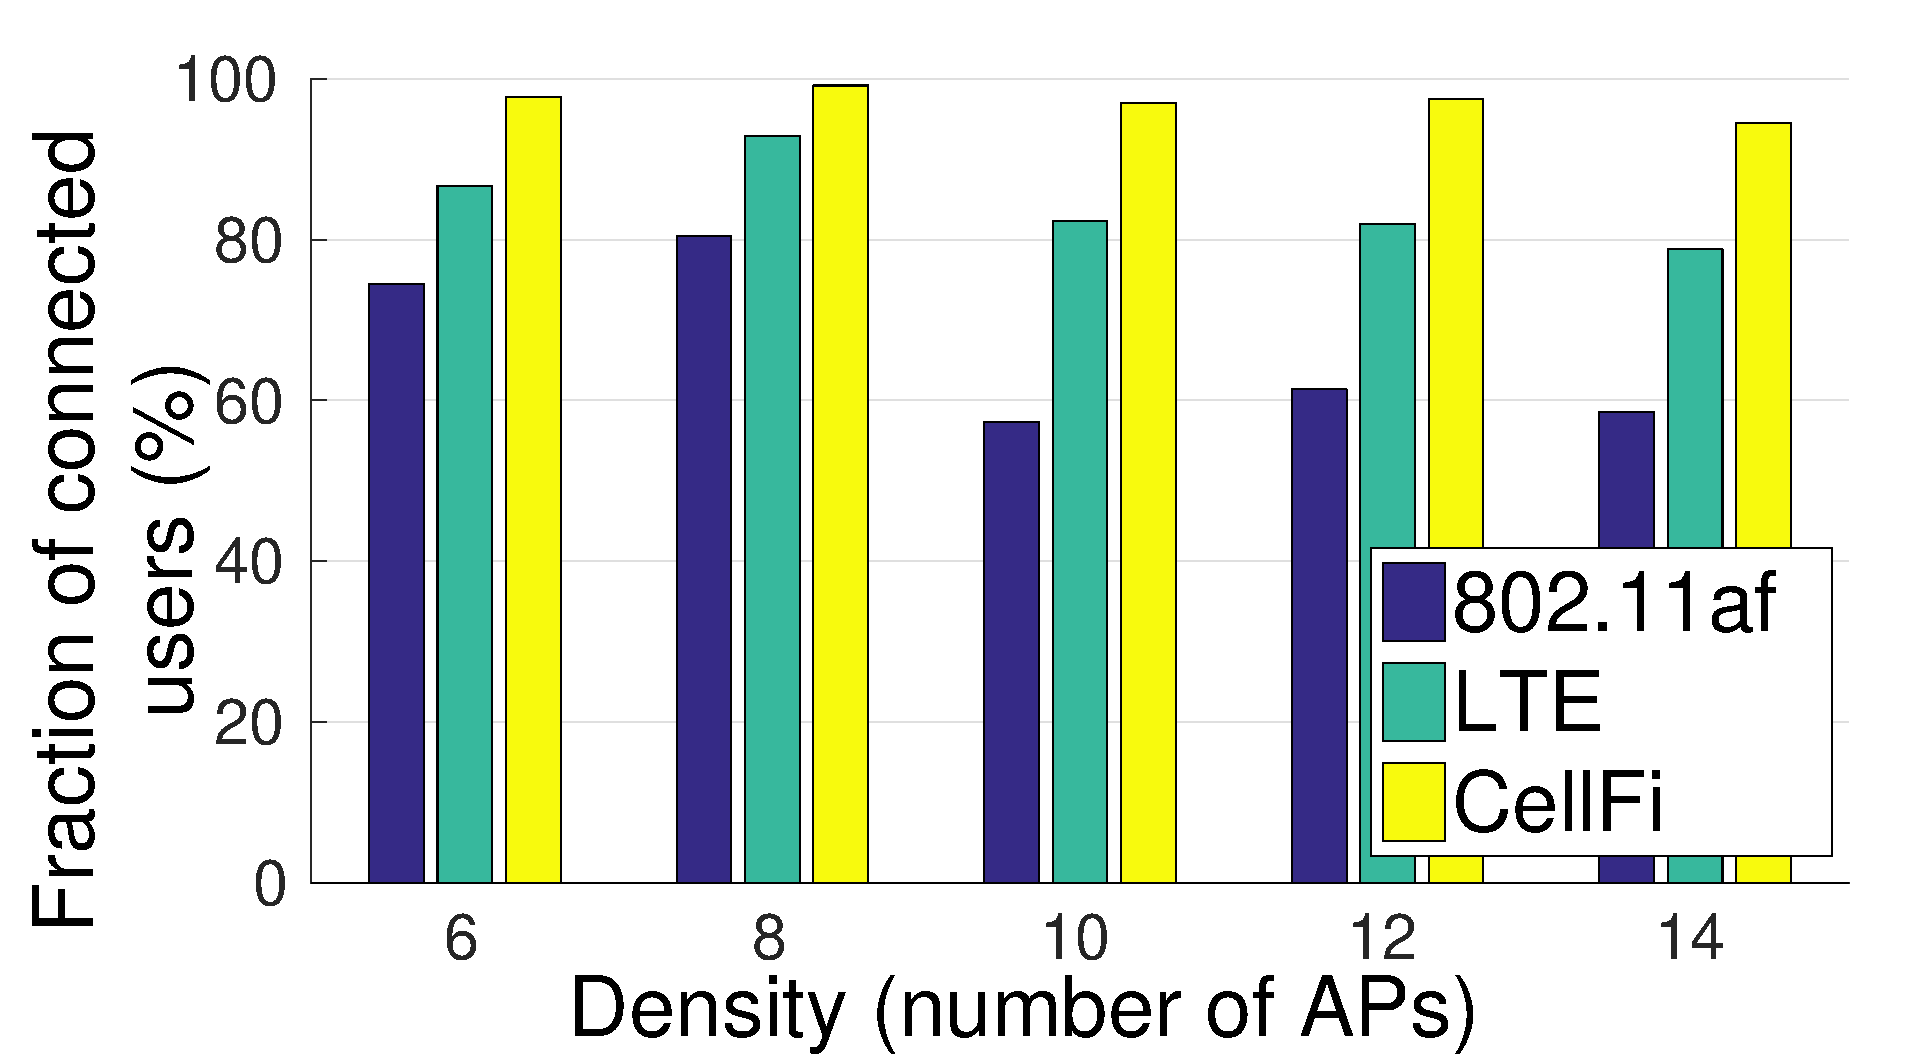
\includegraphics[width=\columnwidth, height=0.38\columnwidth]{./figs/density-crop}
    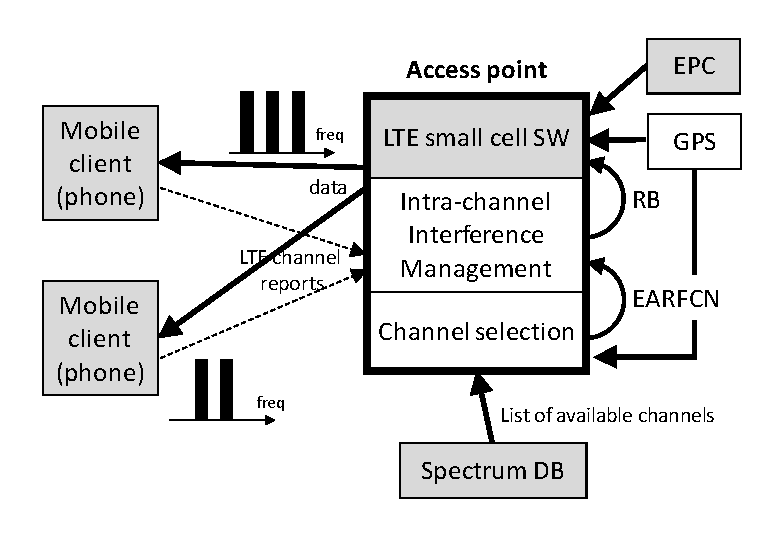
\includegraphics[width=\columnwidth]{./figs/architecture}
    \vspace{-0.3in}
    \caption{\cf architecture overview. The shaded blocks denote unmodified existing components (parts of LTE network stack and TVWS database) and the white blocks are new components introduced by \cf. }
  \label{fig:arch}
\end{figure}

%TWe implement the two new components (interference management and database client) in software. We next explain in detail each of the components and how they interface with the rest of the system.  



\subsection{Channel Selection}

Spectrum access in TV white spaces is managed through a spectrum database~\cite{fcc_db, ofcom_db}. 
The TVWS client in the \cf access point operates by sending the GPS location details to a TVWS database server~\cite{paws},
to which the database responds with a list of available channels (if any), how long then can be used and maximum allowed power levels.  
%There are two types of TVWS client : (i) master client, which in LTE is the access point, and (ii) slave client(s), which in LTE are the mobile devices.
No TVWS client is allowed to transmit in a channel without having a valid lease from a spectrum database and has to stop once a lease has expired.

Satisfying these rules is not straightforward in general. Consider a Wi-Fi client that has associated itself to an AP on a channel with a valid spectrum lease and has gone to sleep. 
In order to be compliant, the client needs to verify the validity of the channel before accessing it next time it has a packet to send, which requires changes to the standard Wi-Fi architecture. 
On the other hand, LTE architecture lends itself to this type of requirements. An LTE client has to get a grant for each uplink transmission from its access point. 
Thus, once an access point looses a spectrum lease and stops transmitting, all of its clients will stop transmitting instantly 
(we demonstrate this in practice for \cf in Section~\ref{sec:database-eval}).

%Furthermore, an LTE access point will only transmit if it has an open SCTP connection to the LTE control plane (EPC). Once this connection is down, the access point will switch the radio off. 

We leverage this observation and build an ETSI-compliant~\cite{etsi_tvws} TVWS database client using the PAWS protocol~\cite{paws}. 
In our architecture there is a single database client that manages both the access point and all its mobile clients, 
and all mobile clients have the same generic location parameters~\cite{etsi_tvws}, determined from the access point's location. 
This is because mobile devices may not have a GPS on the device, or may not be able to get the accurate coordinate (e.g., if located indoors). 

The access point queries for available spectrum for downlink and uplink independently, and then selects the best TV channel that is available for both downlink and uplink and forwards it to the rest of the LTE stack. It is important to keep in mind that the TV white space database is used only to protect incumbents (TV stations and wireless mics), and not to coordinate spectrum among secondary, TV white space devices. 
Instead, \cf uses standard LTE mechanisms such as network listen~\cite{LTEbook} to find an idle channel from the ones offered by the database, if such exists. If not, \cf tries to find a channel that is used by other \cf cells (rather than other non-LTE wireless technologies), as its intra-channel interference mechanism, described next, allows it to gracefully share the channel between other \cf nodes. 

Once a channel is selected, the LTE access points sets the  centre frequency (EARFCN) for downlink transmission and announces the uplink frequency in the LTE SIB control message, both in granularity of 100 kHz~\cite{LTEbullets}. LTE clients are required by standards to be frequency agile and to locate all downlink signals within a wide range of frequencies (e.g., existing LTE bands 41-43 are 200 MHz wide), and are allowed to use only the uplink frequency announced in the SIB messages. 
The database also announces the maximum transmit powers for the corresponding channels; this also gets communicated to the clients through SIB messages. 




\subsection{Intra-channel Interference}
\label{sec:archint}

One of the \cf design goals is to support co-existence between different networks within the same channel.
Conventional LTE access points can coordinate among themselves, using standard protocols (e.g. X2~\cite{LTEbook}), to avoid using the same resource blocks for clients that interfere. This however {\em requires explicit communication and coordination} among access points~\cite{smallcellbook, fermi}. In \cf, coordination is hard to enforce because
 multiple cellular providers are sharing the spectrum and may not even be aware of one another.  
\cf introduces a fully uncoordinated interference management protocol for LTE networks that passively learns about interference from the environment through standard LTE radio procedures, and adapts subchannel allocation accordingly. 
In this way, much like in Wi-Fi, {\em no explicit communication or coordination is required}. 


The essence of \cf's interference management is a short-term resource reservation scheme. 
Each access point runs a distributed algorithm to decide on a set of resource blocks it will use to serve its users and updates the allocation once every 1 second. 
It does not have to be explicitly synchronized with others. 
The intuition for using such long interval (compared to Wi-Fi) is two-fold. 
Firstly, it amortizes the large channel acquisition overheads that arise in long-range networks (Section~\ref{sec:MAC}), which make Wi-Fi inefficient. 
Secondly, such large intervals make sense because LTE also shares a channel in frequency (OFDMA), 
hence multiple users can be served, each on its own set of resource blocks, during 1-second intervals. 
In Section~\ref{sec:eval} we show that this approach has good efficiency with realistic traffic patterns. 

At a high level, the design of the \cf distributed interference management algorithm can be split into two phases.
In the first phase, which we call \emph{distributed share calculation}, 
each node obtains a conservative estimate of its share of the spectrum, 
which is roughly based on its share of clients within the neighborhood.
In the second \emph{distributed subchannel selection} phase, 
nodes attempt to converge towards this share by iterating a randomized contention resolution procedure. 
In this phase, access points attempt to solve an instance of \emph{weighted graph coloring} on the connectivity graph, 
where their weights correspond to their shares.
We discuss these components in more detail in the next section. 


Once the interference management component decides which resource block a scheduler can use, it informs the scheduler using standard interfaces. We don't require any modifications of the standard scheduler. The scheduler is free to schedule any client in any of the resource blocks made available by the interference management system because the interference it creates does not depend on the client selection. This improves spectrum utilization as it allows the scheduler to fully utilize its share of resource blocks by giving all the resources to clients with traffic. 





%\subsection{Interfacing with the rest of the system}
%Standard scheduler, but avoiding black-listed channels.


%% \subsection{Suitability}

%% {\bf We may want to move this part somewhere else:}
%% In this section we argue that the proposed arvhitecture can be implemented with small modifications to the existying LTE hardware and at a low cost. 

%% \noindent{\bf Low cost:}
%% Small cells cost \$1000 and can be much cheaper in high volumes, with transmit powers of up to 30dBm. LTE terminals cost as low as \$50, and can transmit with up to 23dBm. They are also easy to deploy. Small cell E40~\cite{ipa} has dimensions XX. A matching 7dBi antenna costs \$100, has dimensions 25cm x 25cm x 25cm, weights XX kg and can be as easily deployed as a TV antenna.







